\section{Polígono}

O polígono é a lista de vértices em ordem (horária ou anti-horária), com a aresta $p_{n-1} \to p_0$ fechando.

\subsection*{Área}

\smallskip{\centering
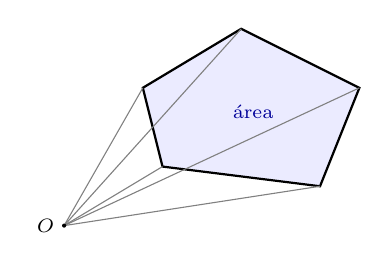
\begin{tikzpicture}[scale=0.5, >=stealth]
  \fill[blue!8] (1,1) -- (5,0.5) -- (6,3) -- (3,4.5) -- (0.5,3) -- cycle;
  \draw[thick] (1,1) -- (5,0.5) -- (6,3) -- (3,4.5) -- (0.5,3) -- cycle;
  \foreach \p in {(1,1), (5,0.5), (6,3), (3,4.5), (0.5,3)} \draw[gray] (-1.5,-0.5) -- \p;
  \fill (-1.5,-0.5) circle (1.5pt) node[left] {\scriptsize $O$};
  \node[blue!60!black] at (3.3,2.4) {\scriptsize área};
\end{tikzpicture}
\par}\smallskip

\texttt{area(p)} soma \texttt{cross(p[i], p[i + 1])}: cada termo é o dobro da área com sinal do triângulo
$O\,p_i\,p_{i+1}$. As partes fora do polígono entram uma vez com cada sinal e se cancelam, e sobra o dobro da área
(positivo se anti-horário). \texttt{area(a, b, c)} é a do triângulo, $|\text{orient}(a, b, c)| / 2$. A soma é exata
com \texttt{T} inteiro; só a divisão por 2 vira real.

\subsection*{Pontos inteiros e Pick}

\smallskip{\centering
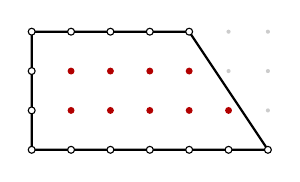
\begin{tikzpicture}[scale=0.5]
  \foreach \i in {0,...,6} \foreach \j in {0,...,3} \fill[gray!40] (\i,\j) circle (1.5pt);
  \draw[thick] (0,0) -- (6,0) -- (4,3) -- (0,3) -- cycle;
  \foreach \p in {(0,0),(1,0),(2,0),(3,0),(4,0),(5,0),(6,0),(4,3),(3,3),(2,3),(1,3),(0,3),(0,1),(0,2)} \draw[fill=white] \p circle (2.5pt);
  \foreach \i in {1,...,4} \foreach \j in {1,...,2} \fill[red!70!black] (\i,\j) circle (2.5pt);
  \fill[red!70!black] (5,1) circle (2.5pt);
\end{tikzpicture}
\par}\smallskip

\texttt{boundary\_points(p)} conta os pontos inteiros na borda (vazados): uma aresta de $p$ até $q$ tem
$\gcd(|dx|, |dy|)$ deles, contando uma das pontas. O teorema de Pick liga a área aos pontos inteiros de um polígono
com vértices inteiros: área $= i + b/2 - 1$, com $i$ pontos dentro (vermelhos) e $b$ na borda. No desenho,
$15 = 9 + 14/2 - 1$. Na prática, o uso mais comum é achar $i = \text{área} - b/2 + 1$.

\subsection*{Ponto dentro}

\smallskip{\centering
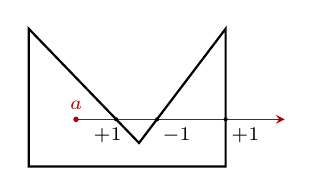
\begin{tikzpicture}[scale=0.5, >=stealth]
  \draw[thick] (0,0) -- (5,0) -- (5,3.5) -- (2.8,0.6) -- (0,3.5) -- cycle;
  \fill[red!70!black] (1.2,1.2) circle (2pt) node[above] {\scriptsize $a$};
  \draw[->, red!70!black] (1.2,1.2) -- (6.5,1.2);
  \foreach \p in {(2.22,1.2), (3.26,1.2), (5,1.2)} \fill \p circle (1.5pt);
  \node at (2.0,0.8) {\scriptsize $+1$};
  \node at (3.75,0.8) {\scriptsize $-1$};
  \node at (5.5,0.8) {\scriptsize $+1$};
\end{tikzpicture}
\par}\smallskip

\texttt{winding\_number(p, a)} conta quantas voltas o polígono dá em torno de $a$: anda por um raio saindo de $a$ para
a direita e soma $+1$ quando uma aresta o cruza subindo e $-1$ quando cruza descendo. Diferente de zero se $a$ está
dentro, zero se está fora ou na borda. É exato com \texttt{T} inteiro e funciona para qualquer polígono, convexo ou
não.

\subsection*{Fecho convexo}

\smallskip{\centering
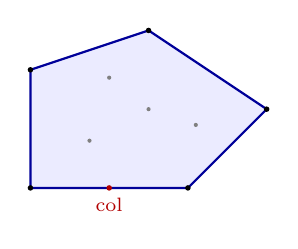
\begin{tikzpicture}[scale=0.5]
  \fill[blue!8] (0,0) -- (4,0) -- (6,2) -- (3,4) -- (0,3) -- cycle;
  \draw[thick, blue!60!black] (0,0) -- (4,0) -- (6,2) -- (3,4) -- (0,3) -- cycle;
  \foreach \p in {(0,0), (4,0), (6,2), (3,4), (0,3)} \fill \p circle (2pt);
  \foreach \p in {(1.5,1.2), (3,2), (4.2,1.6), (2,2.8)} \fill[gray] \p circle (1.5pt);
  \fill[red!70!black] (2,0) circle (2pt) node[below] {\scriptsize col};
\end{tikzpicture}
\par}\smallskip

\texttt{convex\_hull(p, col)} devolve o menor polígono convexo que contém todos os pontos, em sentido anti-horário a
partir do menor ponto. Ordena os pontos e monta a metade de baixo e depois a de cima, tirando o último ponto sempre que
ele faz uma curva para a direita. Com \texttt{col} verdadeiro, mantém os pontos no meio das arestas (como o vermelho);
se todos forem colineares, devolve todos em ordem.

\subsection*{Ponto em polígono convexo}

\smallskip{\centering
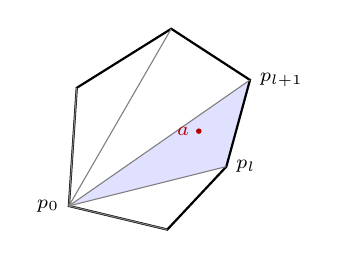
\begin{tikzpicture}[scale=0.5]
  \fill[blue!12] (0,0) -- (4,1) -- (4.6,3.2);
  \draw[thick] (0,0) -- (2.5,-0.6) -- (4,1) -- (4.6,3.2) -- (2.6,4.5) -- (0.2,3) -- cycle;
  \foreach \p in {(2.5,-0.6), (4,1), (4.6,3.2), (2.6,4.5), (0.2,3)} \draw[gray] (0,0) -- \p;
  \node[left] at (0,0) {\scriptsize $p_0$};
  \node[right] at (4,1) {\scriptsize $p_l$};
  \node[right] at (4.6,3.2) {\scriptsize $p_{l+1}$};
  \fill[red!70!black] (3.3,1.9) circle (2pt) node[left] {\scriptsize $a$};
\end{tikzpicture}
\par}\smallskip

\texttt{in\_convex(p, a)} responde em $O(\log n)$: as diagonais a partir de $p_0$ dividem o polígono em triângulos em
leque, e uma busca binária com \texttt{orient} acha o triângulo $p_0\,p_l\,p_{l+1}$ onde $a$ cairia. Basta testar o
lado de $a$ em relação à aresta $p_l \to p_{l+1}$. Devolve $1$ dentro, $0$ na borda e $-1$ fora. O polígono precisa
ser estritamente convexo e anti-horário, como sai do \texttt{convex\_hull(p, false)}.

\subsection*{Par mais distante}

\smallskip{\centering
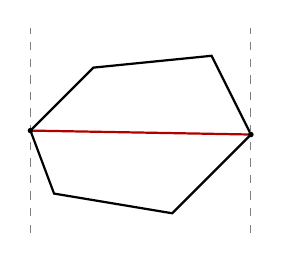
\begin{tikzpicture}[scale=0.5]
  \draw[thick] (0,0) -- (3,-0.5) -- (5,1.5) -- (4,3.5) -- (1,3.2) -- (-0.6,1.6) -- cycle;
  \draw[gray, dashed] (-0.6,-1) -- (-0.6,4.2);
  \draw[gray, dashed] (5,-1) -- (5,4.2);
  \draw[red!70!black, thick] (-0.6,1.6) -- (5,1.5);
  \fill (-0.6,1.6) circle (2pt);
  \fill (5,1.5) circle (2pt);
\end{tikzpicture}
\par}\smallskip

\texttt{farthest\_pair(p)} devolve a maior distância ao quadrado entre dois pontos. O par mais distante está no fecho
convexo, e para cada aresta do fecho o ponto mais longe dela (o par de ``pinças'' paralelas tracejadas) só anda para
a frente enquanto as arestas giram. Por isso o laço é $O(n)$ depois do fecho. Exato com \texttt{T} inteiro.

\subsection*{Corte por uma reta}

\smallskip{\centering
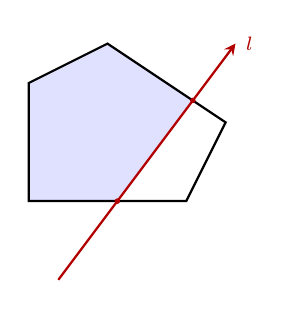
\begin{tikzpicture}[scale=0.5, >=stealth]
  \fill[blue!12] (0,0) -- (2.25,0) -- (4.167,2.556) -- (2,4) -- (0,3) -- cycle;
  \draw[thick] (0,0) -- (4,0) -- (5,2) -- (2,4) -- (0,3) -- cycle;
  \draw[->, red!70!black, thick] (0.75,-2) -- (5.25,4) node[right] {\scriptsize $l$};
  \fill[red!70!black] (2.25,0) circle (2pt);
  \fill[red!70!black] (4.167,2.556) circle (2pt);
\end{tikzpicture}
\par}\smallskip

\texttt{polygon\_cut(p, l)} devolve a parte do polígono convexo à esquerda de $l$ (\texttt{side} $\ge 0$, em azul):
anda pelas arestas guardando os vértices desse lado e, quando uma aresta atravessa a reta, o ponto de travessia. Cortar
um polígono convexo por todas as arestas de outro dá a interseção dos dois. Exige \texttt{T} real.

\subsection*{Soma de Minkowski}

\smallskip{\centering
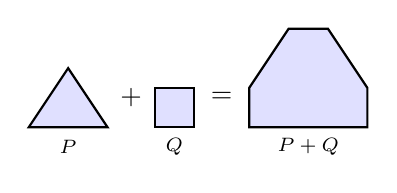
\begin{tikzpicture}[scale=0.5]
  \draw[thick, fill=blue!12] (0,0) -- (2,0) -- (1,1.5) -- cycle;
  \node at (1,-0.5) {\scriptsize $P$};
  \node at (2.6,0.75) {$+$};
  \draw[thick, fill=blue!12] (3.2,0) -- (4.2,0) -- (4.2,1) -- (3.2,1) -- cycle;
  \node at (3.7,-0.5) {\scriptsize $Q$};
  \node at (4.9,0.75) {$=$};
  \draw[thick, fill=blue!12] (5.6,0) -- (8.6,0) -- (8.6,1) -- (7.6,2.5) -- (6.6,2.5) -- (5.6,1) -- cycle;
  \node at (7.1,-0.5) {\scriptsize $P + Q$};
\end{tikzpicture}
\par}\smallskip

\texttt{minkowski(p, q)} é o polígono de todas as somas $a + b$, com $a$ em $P$ e $b$ em $Q$. As arestas dele são as
arestas de $P$ e de $Q$ intercaladas em ordem de ângulo, então basta começar dos dois menores vértices e ir somando,
escolhendo a próxima aresta pelo sinal do \texttt{cross} (como no merge do merge sort). Serve para distância entre
polígonos convexos e para testar colisão (verificar se $P + (-Q)$ contém a origem). Exato com \texttt{T} inteiro; os
dois polígonos precisam ser estritamente convexos e anti-horários.
